\PassOptionsToPackage{brazil,american}{babel}
\documentclass[12pt]{article}

\usepackage{sbc-template}
\usepackage[brazil,american]{babel}
\usepackage[utf8]{inputenc}

\usepackage{graphicx}
\usepackage{url}
\usepackage{float}
\usepackage{listings}	
\usepackage{color}
\usepackage{todonotes}
\usepackage{algorithmic}
\usepackage{algorithm}
\usepackage{hyperref}
\usepackage{amsmath}
\usepackage{tikz}
\newcommand\net{%
	\begin{tikzpicture}[scale=0.3\baselineskip/18pt]
	\draw (0,1) -- (1,1) -- (1,0) -- (2,0);
	\end{tikzpicture}%
}

\newcommand\netp{%
	\begin{tikzpicture}[scale=0.3\baselineskip/18pt]
	\draw (0,1) -- (1,1) -- (1,0) -- (2,0) -- (2,1) -- (3,1);
	\end{tikzpicture}%
}


\sloppy

\title{Experimento 8\\ 
	FLIP-FLOPS:RS E JK}

\author{
	Lucas Mafra Chagas, 12/0126443 \\
	Marcelo Giordano Martins Costa de Oliveira,  12/0037301
}


\address{Dep. Ciência da Computação -- Universidade de Brasília (UnB)\\
	CiC 116351 - Circuistos Digitais - Turma C
	\email{\{giordano.marcelo, chagas.lucas.mafra\}@gmail.com}
}

\begin{document} 

\maketitle

 \begin{abstract}
	 In this experiment, we will study some types of flip-flops RS and JK by implementing, verifying their truth tables and comparing with the theoretical well-known results.
 \end{abstract}
     
 \begin{resumo} 
	 Neste experimento, serão estudados os alguns tipos de flip-flops RS e JK, através de sua implementação e posterior verificação de suas respectivas tabelas verdade, comparando-as com os resultados esperados teoricamente.
 \end{resumo}


\section{Objetivos}
\label{sec:Objetivos}

Apresentação do flip-flop como unidade armazenadora de memória. Observação do funcionamento e construção dos flip-flops RS, RS Gatilhado, SENHOR-ESCRAVO e JK SENHOR-ESCRAVO.

\section{Materiais} 
\label{sec:Materiais}

\begin{itemize}
    \item Painel Digital
    
    \item \textit{protoboard}
    
    \item Fios
    
    \item Portas Lógicas NAND, NOR e NOT.
    
\end{itemize}


\section{Introdução}
\label{sec:Introducao}

O flip-flop, ou multivibrador biestável, é um circuito digital pulsado capaz de servir como uma memória de um bit. Um flip-flop tipicamente tem dois sinais de entrada, o \textit{SET} e o \textit{RESET}, um sinal de clock (gatilho), um sinal de saída e o seu inverso. A pulsação ou mudança no sinal do clock faz com que o flip-flop mude ou retenha seu sinal de saída, baseado nos valores dos sinais de entrada e na equação característica do flip-flop. Existem vários tipos de flip-flops.

\subsection{Flip-flop Latch RS}
O valor guardado no flip-flop será mantido se \textit{SET} e \textit{RESET} forem ambos iguais a 0; irá mudar para 0, se a entrada \textit{RESET} for 1, e se tornará 1 se a entrada \textit{SET} for 1. O comportamento não será especificado se as duas entradas forem iguais a 1. Esse comportamento, neste relatório será referido como o estado proibido. Aqui temos uma implementação desse flip-flop feito apenas com portas NAND.

\begin{figure}[H]
	\centering
	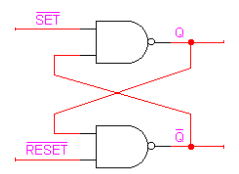
\includegraphics[width=.5\textwidth]{latchRS.png}
	\caption{Latch RS}
	\label{fig:latRS}
\end{figure}

Para este tipo de implementação temos que considerar que a ativação de \textit{SET} ou \textit{RESET} é feita quando a entrada é 0. Além disso, temos que para esse flip-flop a saída possui um complemento, que sempre será o inverso da saída original.

\subsection{Flip-Flop RS Gatilhado}

Aqui há a inclusão de um gatilho(toggle) T. Quando houver variação do clock, o valor guardado no flip-flop será alternado ou mantido dependendo se o valor na entrada T (gatilho), se ele está em 1 ou 0. Se o valor de T é 1 temos que o valor será alterado de acordo com as entradas em \textit{SET} e \textit{RESET}. Se o valor de T é 0, o último valor alterado será armazenado, pois \textit{$\overline{SET}$} e \textit{$\overline{RESET}$} serão ambos iguais a 0. Portanto, a cada pulso de T temos o armazenamento da última mudança feita no flip-flop.

\begin{figure}[H]
	\centering
	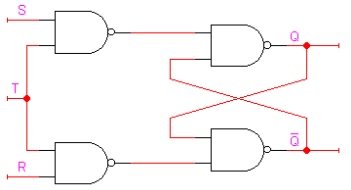
\includegraphics[width=.5\textwidth]{RSgat.png}
	\caption{Latch RS Gatilhado}
	\label{fig:RSgat}
\end{figure}

Para este flip-flop temos também a entrada proibida. Se ambos o \textit{SET} e o \textit{RESET} estiverem ativados, a saída será indeterminada.


\subsection{Flip-Flop RS Gatilhado com PRESET e CLEAR}

Este flip-flop é um Flip-Flop RS Gatilhado mas que pode forçar um resultado desejado na saída Q, já que as entradas \textit{RESET} e \textit{CLEAR} funcionam independentemente do gatilho T e das entradas \textit{SET} e \textit{RESET}.

\begin{figure}[H]
	\centering
	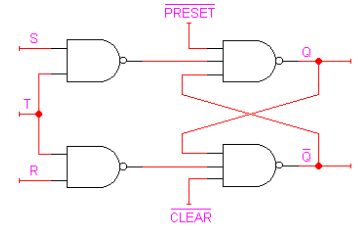
\includegraphics[width=.5\textwidth]{RSgatPC.png}
	\caption{Latch RS Gatilhado com PRESET e CLEAR}
	\label{fig:RSgatPC}
\end{figure}

\subsection{Flip-Flop SENHOR-ESCRAVO}

Este flip-flop é a junção de dois flip-flops RS Gatilhados. As saídas do primeiro flip-flop são as entradas do segundo. O gatilho T porém, nunca possui o mesmo valor nos diferentes flip-flops. Se o gatilho é 1 no flip-flop SENHOR, temos que os valores neste flip-flop podem ser alterados mas o flip-flop ESCRAVO, que terá seu gatilho em 0 permanecerá em repouso. Quando desligamos o gatilho do flip-flop SENHOR, acionamos o escravo, que pegará a informação armazenada no senhor e a armazenará também. Portanto, a cada pulso do gatilho temos que o valor no flip-flop SENHOR será alterado e essa alteração será transferida para o ESCRAVO.

\begin{figure}[H]
	\centering
	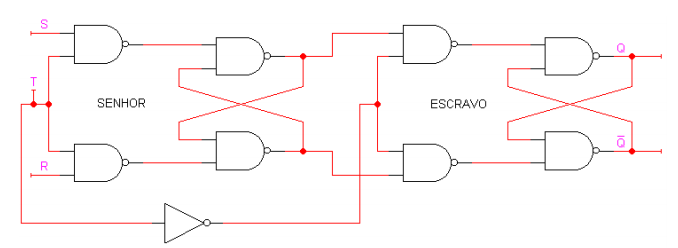
\includegraphics[width=.5\textwidth]{ffMS.png}
	\caption{Flip-Flop SENHOR-ESCRAVO (Master-Slave)}
	\label{fig:ffMS}
\end{figure} 

\subsection{Flip-Flop JK SENHOR-ESCRAVO}

Este flip-flop permite a utilização do antes estado proibido. Temos que quando houver variação do clock, o valor guardado no flip-flop será alternado se as entradas J e K forem ambas iguais a 1 e será mantido se ambas forem iguais a zero. Se forem diferentes, haverá o \textit{SET} ou o \textit{RESET} dos valores.

\begin{figure}[H]
	\centering
	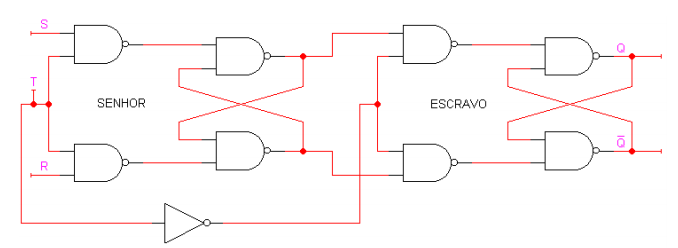
\includegraphics[width=.5\textwidth]{ffJKMS.png}
	\caption{Flip-Flop JK SENHOR-ESCRAVO (Master-Slave)}
	\label{fig:ffJKMS}
\end{figure} 

\section{Procedimentos}
\label{sec:Procedimentos}

O relatório é dividido em 5 etapas:

\begin{itemize}
	\item Montar o circuito Latch RS com portas NAND
	\item Montar o circuito Latch engatilhado
	\item Montar o circuito Latch engatilhado com entradas PRESET e CLEAR
	\item Montar o circuito de um flip-flop RS MESTRE-ESCRAVO usando portas NAND’s
	\item Montar o circuito de um flip-flop JK MESTRE-ESCRAVO
\end{itemize}

Esse experimento é montado de forma gradual, assim um circuito está diretamente ligado ao outro.

\subsection{Implementação de um circuito Latch RS com portas NAND}
\label{sec:2.1}

\begin{figure}[H]
	\centering
	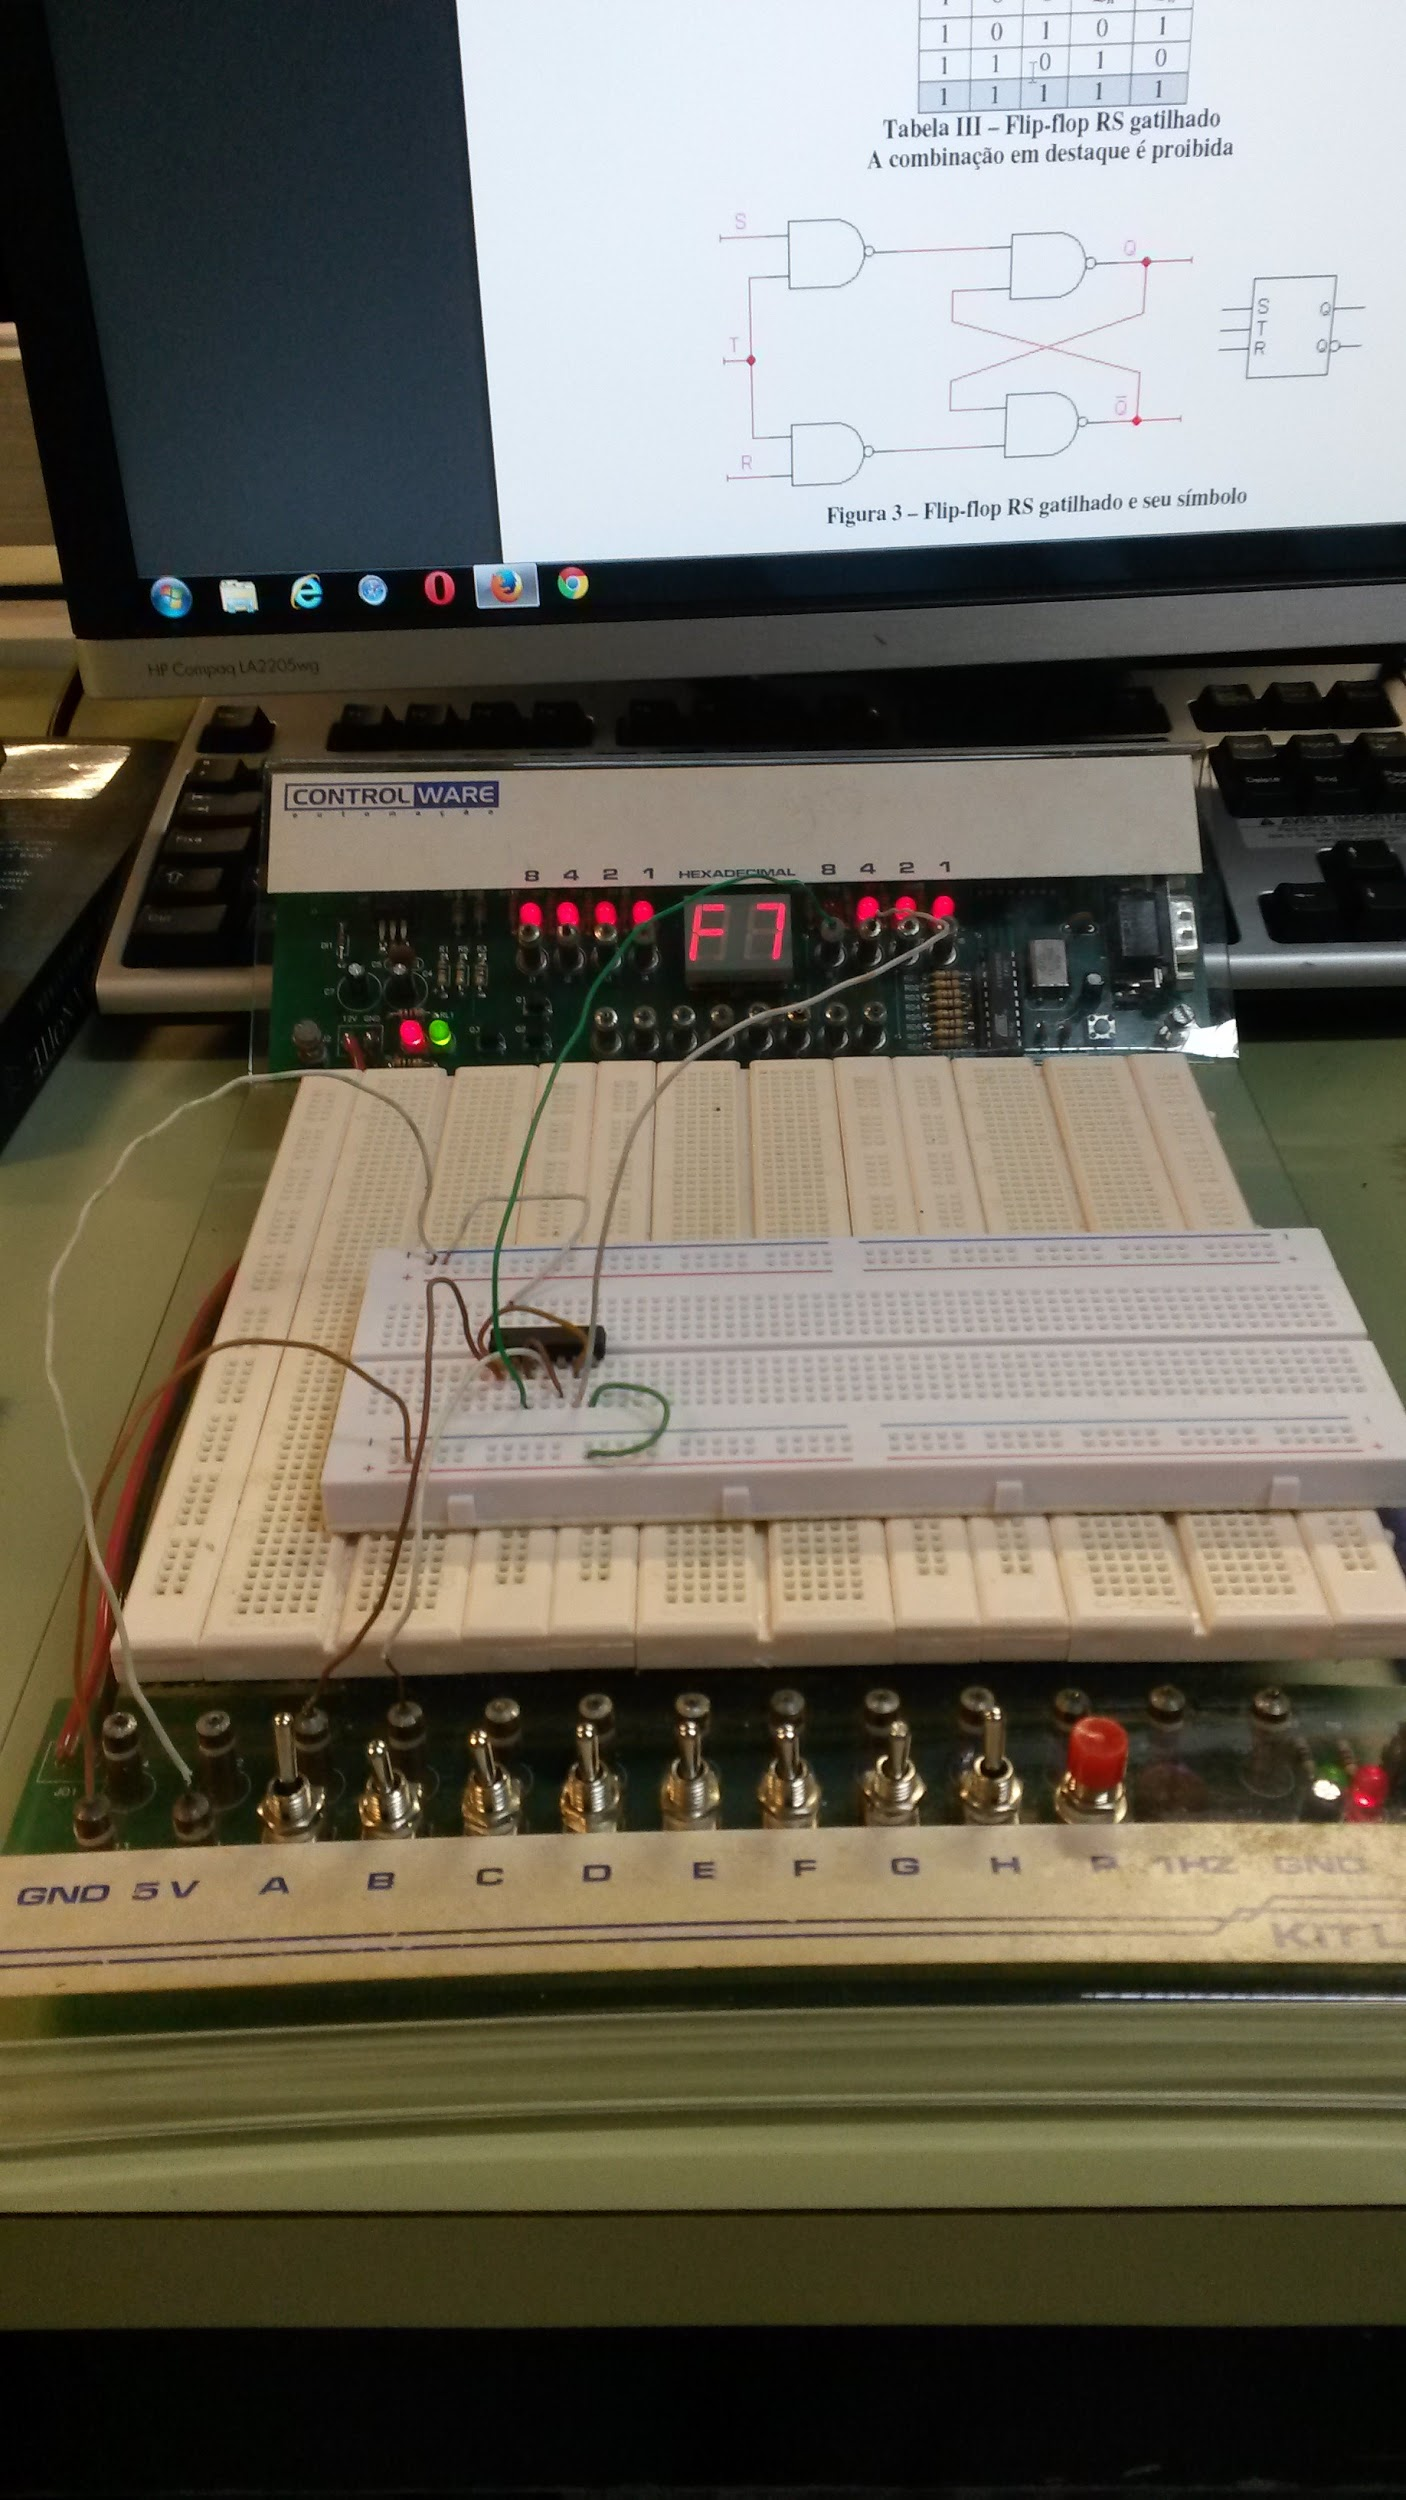
\includegraphics[width=.5\textwidth]{latchRSNAND.png}
	\caption{Latch RS utilizando portas NAND}
	\label{fig:lRSNAND}
\end{figure}

Resultados obtidos para Q e $\overline{Q}$ para a sequência 10,11,01,11,00,11 de $\overline{SET}$ e $\overline{RESET}$

Observação: para este flip-flop temos que o $\overline{SET}$ e o $\overline{RESET}$ estão ativados em nível 0 ao invés de nível 1. Para as outras partes do experimento temos o caso oposto.

\begin{table}[H]
	\centering
	\begin{tabular}{|c|c|c|c|}
		\cline{1-4}
		\multicolumn{1}{|c|}{S} & \multicolumn{1}{|c|}{R} & \multicolumn{1}{|c|}{Q} & \multicolumn{1}{|c|}{$\overline{Q}$} \\
		\hline
		1 & 0 & 0 & 1  \\
		\hline
		1 & 1 & 0 & 1 \\
		\hline
		0 & 1 & 1 & 0  \\
		\hline
		1 & 1 & 1 & 0  \\
		\hline
		0 & 0 & 1 & 1  \\
		\hline
		1 & 1 & 0 & 1  \\
		\hline
	\end{tabular}
	\caption{Tabela-Verdade do Latch RS}
\end{table}

Vemos que quando $\overline{RESET}$ está ativado, temos que a saída Q é igual a 0 e a saída $\overline{Q}$ é igual a 1. Ao desligarmos o $\overline{RESET}$, deixando ambos o $\overline{SET}$ e o $\overline{RESET}$ em repouso, temos que o flip-flop mantém essa configuração das saídas armazenadas. Esse armazenamento também ocorre quando ativamos o $\overline{SET}$ e desativamos o $\overline{RESET}$. A única diferença é que neste caso, Q é 1 e $\overline{Q}$ é 0. Finalmente, quando ativamos ambos $\overline{SET}$ e $\overline{RESET}$ temos o estado proibido onde tanto Q como $\overline{Q}$ são iguais a 1, o que é uma incoerência. Ao desligarmos as chaves após o estado proibido, temos Q e $\overline{Q}$ apresentando um resultado qualquer. 
A partir disso, vemos que a tabela verdade obtida para este circuito é:

\begin{table}[H]
	\centering
	\begin{tabular}{|c|c|c|c|}
		\cline{1-4}
		\multicolumn{1}{|c|}{S} & \multicolumn{1}{|c|}{R} & \multicolumn{1}{|c|}{$Q_{n+1}$} & \multicolumn{1}{|c|}{$\overline{Q_{n+1}}$} \\
		\hline
		0 & 0 & 1 & 1  \\
		\hline
		0 & 1 & 1 & 0 \\
		\hline
		1 & 0 & 0 & 1  \\
		\hline
		1 & 1 & $Q$ & $\overline{Q}$  \\
		\hline
	\end{tabular}
	\caption{Tabela-Verdade do Latch RS}
\end{table}


\subsection{Implementação de um circuito Latch gatilhado}
\label{sec:2.2}

\href{https://youtu.be/azJt3y337BE}{Vídeo 2.2}

Vemos pelo vídeo que quando o gatilho T está desligado, ele armazena o último valor de Q e $\overline{Q}$ que foram inseridos, independente do ativamento ou desativamento de $\overline{SET}$ e $\overline{RESET}$. Antes de T estar desligado, tínhamos a chave RESET acionada, por isso que Q era 0 e $\overline{Q}$ era 1. Já quando temos T ativado, ou seja, acionado em 1, temos que o alterando SET e RESET obtemos os mesmos valores da tabela verdade em ~\ref{sec:2.1}. Temos portanto que T define se o flip-flop está em repouso ou se ele está recebendo informação. Quando T é igual a 0 e o flip-flop está em repouso, temos que a saída referente à última entrada aplicada fica retida dentro do flip flop. Ficamos, portanto, com a seguinte tabela verdade:

\begin{table}[H]
	\centering
	\begin{tabular}{|c|c|c|c|c|}
		\cline{1-5}
		\multicolumn{1}{|c|}{T} & \multicolumn{1}{|c|}{S} & \multicolumn{1}{|c|}{R} & \multicolumn{1}{|c|}{$Q_{n+1}$} & \multicolumn{1}{|c|}{$\overline{Q_{n+1}}$} \\
		\hline
		0 & X & X & $Q_{n}$ & $\overline{Q_{n}}$  \\
		\hline
		1 & 0 & 0 & $Q_{n}$ & $\overline{Q_{n}}$  \\
		\hline
		1 & 0 & 1 & 0 & 1 \\
		\hline
		1 & 1 & 0 & 1 & 0  \\
		\hline
		1 & 1 & 1 & 1 & 1  \\
		\hline
	\end{tabular}
	\caption{Tabela-Verdade do Latch gatilhado}
\end{table}

\subsection{Implementação flip-flop RS SENHOR-ESCRAVO com portas NAND}
\label{sec:2.3}

\href{https://youtu.be/c2MW7RQl_7s}{Vídeo 2.3}

Após construído o circuito, para cada possível entrada das chaves $SET$ e $RESET$ foi observada a saída do ESCRAVO após cada pulso aplicado em T. A análise foi feita a partir de pulsos pois para este tipo de circuito quando temos T=0, temos a informação sendo passada do flip-flop SENHOR para o flip-flop ESCRAVO e quanto T=1 temos que o flip-flop ESCRAVO aguarda enquanto alteramos valores no flip-flop SENHOR, e queríamos fazer a observação do que o flip-flop armazenava após uma mudança(um pulso) completo. A partir disso, constroi-se a seguinte tabela verdade:

\begin{table}[H]
	\centering
	\begin{tabular}{|c|c|c|c|c|}
		\cline{1-5}
		\multicolumn{1}{|c|}{T} & \multicolumn{1}{|c|}{S} & \multicolumn{1}{|c|}{R} & \multicolumn{1}{|c|}{$Q_{n+1}$} & \multicolumn{1}{|c|}{$\overline{Q_{n+1}}$} \\
		\hline
		0 & X & X & $Q_{n}$ & $\overline{Q_{n}}$  \\
		\hline
		pulse & 0 & 0 & $Q_{n}$ & $\overline{Q_{n}}$  \\
		\hline
		pulse & 0 & 1 & 0 & 1 \\
		\hline
		pulse & 1 & 0 & 1 & 0  \\
		\hline
		pulse & 1 & 1 & 1 & 1  \\
		\hline
	\end{tabular}
	\caption{Tabela-Verdade do Flip-flop SENHOR-ESCRAVO}
\end{table}
pulse = \netp~

Vemos pela tabela e pelas imagens que o escravo armazenava o valor após o fim do pulso, alterado quando T = 1. Temos portanto, que a construção deste flip-flop teve sucesso.

\subsection{Implementação de um flip-flop JK SENHOR-ESCRAVO com portas NAND}
\label{sec:2.4}

Com base na imagem abaixo e reutilizando os flip-flops construídos anteriormente, devia-se montar o circuito de um flip-flop JK SENHOR-ESCRAVO.

\begin{figure}[H]
	\centering
	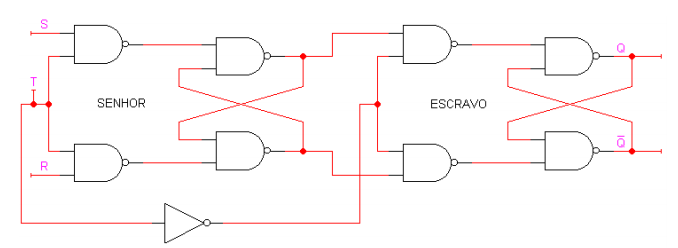
\includegraphics[width=.5\textwidth]{ffJKMS.png}
	\caption{Flip-Flop JK SENHOR-ESCRAVO (Master-Slave)}
	\label{fig:ffJKMS}
\end{figure} 

E sua tabela deveria ser:

\begin{figure}[H]
	\centering
	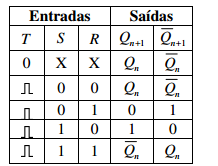
\includegraphics[width=.5\textwidth]{tvjkms.png}
	\caption{Tabela verdade do Flip-Flop JK SENHOR-ESCRAVO (Master-Slave)}
	\label{fig:tvJKMS}
\end{figure}

Mas, infelizmente, por conta de alguns fios com problemas, não conseguimos finalizar essa parte.


\section{Análise dos Resultados}
\label{sec:Resultados}

Analisando os dados da sessão ~\ref{sec:2.1} à ~\ref{sec:2.3}, conseguimos comparar as tabelas verdades resultantes do experimento com as tabelas fornecidas pelo roteiro do experimento 8, mesmo que não tenhamos conseguido terminar a parte ~\ref{sec:2.4}, a maior parte dos resultados está dentro dos conformes, portanto, consideramos o experimento um sucesso.
\section{Conclusão}
\label{sec:Conclusao}

Neste experimento foi possível perceber a importância de um flip-flop na utilização de armazenamento de informações. Vimos que, se construídos corretamente, os flip-flops podem ser úteis em diversas aplicações

\newpage 
% Colocar aqui apenas as respostas dos itens da Auto-Avaliação
\section*{Auto-Avaliação}

\begin{enumerate}
    \item d
    \item a
    \item d
    \item d
    \item c
    \item a
    \item a
\end{enumerate}


\end{document}
